\documentclass{llncs}
\usepackage{graphicx}
\usepackage{wrapfig}

\title{Implementation of a template system with semantic web services}
\author{Adan Scotney\thanks{This work is supported by the IST ALIVE project} \small{(\emph{a.scotney@bath.ac.uk})}}
\institute{University of Bath}

\begin{document}
\maketitle
\begin{abstract}
 OWL-S supports the concept of composite services. In these services, a data 
 flow is defined to allow execution of multiple services as a single one. 
 However, the processes which make up this composite services are static. Once 
 the flow has been defined, that is final. This tool, developed as part of the 
 ALIVE \cite{alive} project, allows one to ground templates, composites where the concrete 
 implementation of a particular process is undefined, to form an invokable 
 composite service.
\end{abstract}
\section{Introduction}
 OWL-S \cite{owls} composite services provide a way of combining multiple services into a 
 single one. Ordinarily, the services which make up the composite are fixed, 
 but using the concept of templates, it is possible to replace the processes 
 which make up a composite, while leaving the data flow in tact.

 The concept of a template is simple: a composite service where one or more of 
 the sub-processes are not invokable. These sub-processes are called slots if 
 they have inputs and outputs (bound to inputs and outputs in the outer 
 composite as normal), but no concrete process is pointed to.

\begin{figure}[htb]
\vspace{-15pt}
\begin{center}
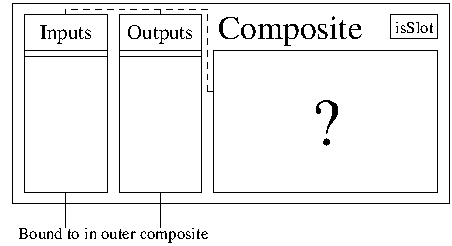
\includegraphics[width=3.5in]{slotDiagram}
\caption{A slot}
\end{center}
\vspace{-25pt}
\end{figure}

 In this implementation, slots are themselves composite processes, which are 
 sub-processes of the outer composite. They have inputs and outputs bound to 
 the outer process, a slot marker, and an empty ControlConstruct.

 When grounding a slot, a Perform is built within the slot process, which 
 contains the grounded process, and bindings are then built to this from the 
 slot inputs and outputs, allowing it to be invoked as if the parameters passed 
 between the slot and outer composite were in fact passed directly to the 
 grounded process.

\begin{figure}[htb]
\vspace{-15pt}
\begin{center}
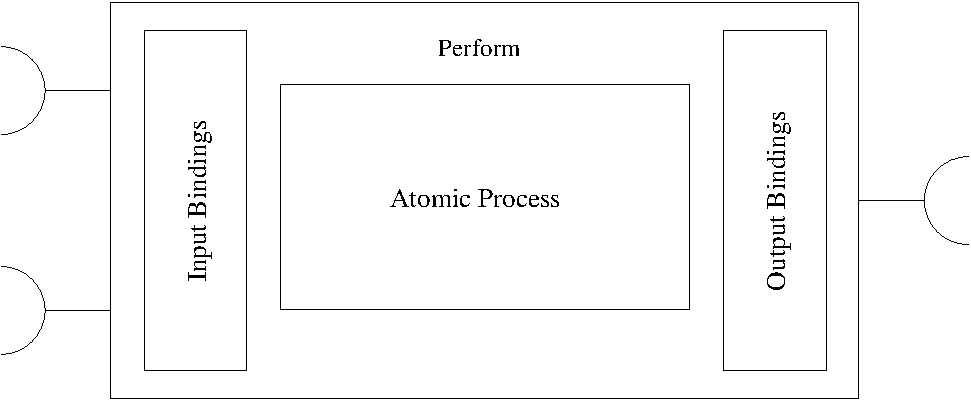
\includegraphics[width=3.5in]{perform}
\caption{The constructed perform which is inserted into a slot}
\end{center}
\vspace{-25pt}
\end{figure}

 In addition to simply grounding templates, the API also provides a mechanism 
 for accessing the ALIVE matchmaker to discover candidates, and another for 
 setting constraints upon the services which can be selected by using ASP 
 (Answer Set Programming) \cite{potassco}.

\section{Creating a template}
 When creating a template, there are three properties which are defined 
 in the included templates ontology
 (\texttt{http://www.ist-alive.eu/ontologies/ALIVE-Template.owl}) that 
 must be used. These are as follows:
 \begin{itemize}
 	\item \texttt{isSlot} on \texttt{CompositeProcess} : Datatype property 
 		containing a string which is the identifier of the slot. This
 		must be a valid ASP name (i.e. lower case, no spaces). A 
 		composite process which has this property is considered a slot.
 	\item \texttt{aspCode} on \texttt{Service} : Datatype property containing 
 		a string, which is used to select possible services with ASP. See 
 		the ASP section below.
 	\item \texttt{aspBindings} on \texttt{Service} : Datatype property containing 
 		a string for user-defined ASP bindings. See the ASP section below.
 \end{itemize}

 To create a template, simply create a service as described above, then assert each 
 oh these properties where appropriate. There should only be one \texttt{aspCode} and 
 one \texttt{aspBindings} on the Service, and at least one \texttt{CompositeService} 
 as a sub-process of the main service which is labelled with \texttt{isSlot}.

 This proved to be the most workable approach, after attempts were made to use 
 atomic processes as slots, directly swapping them out and rebuilding the bindings; and 
 also to make the replacement service and parameters \texttt{owls:sameAs} those of the 
 slot.

\section{API Use}
\subsection{API Configuration}
 The API uses some Java properties which define how it generates answer sets. 
 These are ordinarily contained within the \texttt{alivetemplates.properties} 
 file, however there are forms of the \texttt{TemplateConstructorImpl} 
 constructor which take a Properties object as a parameter, allowing one to 
 use the API where it isn't possible to determine where the file should be 
 located.

 \begin{itemize}
 	\item \texttt{clingopath} : Path to the clingo binary.
 	\item \texttt{clingoargs} : Arguments to pass when invoking clingo (number of answer sets generated can be limited here).
 \end{itemize}

 It is also possible to override the path of the properties file by setting 
 the \texttt{aspconfig.file} system property.

\subsection{Interface}
 The API is accessible through an interface, \texttt{TemplateConstructor} of which 
 \texttt{TemplateConstructorImpl} is the included implementation. Full details of 
 the interface can be found in the Javadocs, however it will be briefly outlined 
 here.

 \begin{itemize}
 	\item \texttt{List<Process> findTemplateSlots()} Helper method to find all slots.
	\item \texttt{Map<Process, Collection<Match>> getCandidates(List<Process> slotProcesses)} Invokes the matchmaker on a list of slots, and 
 		returns a Map from slots to a collection of matches (services which have compatible inputs and outputs).
	\item \texttt{Program getGeneratedASP(Map<Process, Collection<Match>> candidates)} Fetches the answer set program which will 
 		be used to select which processes can fit into each slot. This can be used to add additional assertions outside of 
 		the API should you wish.
	\item \texttt{List<TemplateAnswerSet> getAnswerSets(Program aspProg)} Runs an answer set program and returns the sets of 
 		processes which can be used, along with the original model returned from clingo, allowing one to extract 
 		additional information which the API doesn't look for.
	\item \texttt{OWLOntology performReplacement(Map<Process, Process> replacements, URI newServiceURI)} Returns an ontology 
 		containing the template as a service grounded with the specified URI.
 \end{itemize}

There are some additional methods which can be found in the Javadocs, but these 
are the core ones required to use the API.

\subsection{Example}

A short example of the way in which one may typically use the API.

\begin{verbatim}
TemplateConstructor builder = new TemplateConstructorImpl(
   new File("test/newcomp.owl").toURI(), 
   URI.create("urn:test-composite-ont#MasterService"), matchMaker);
		
// Run template
List<Process> slotList = builder.findTemplateSlots();
Map<Process, Collection<Match>> candidateMap = builder.getCandidates(slotList);
Program aspProg = builder.getGeneratedASP(candidateMap);
List<TemplateAnswerSet> selectionMaps = builder.getAnswerSets(aspProg);
OWLOntology ont = builder.performReplacement(selectionMaps.get(1).getMapping(),
   URI.create("urn:test-composite-ont#GroundedMasterService"));
// Store result
ont.write(new FileOutputStream(new File("groundedTemplate.owl")), 
   URI.create("urn:alive-templates"));
\end{verbatim}

\section{ASP}
\subsection{Outline}
 The templates API allows the programmer to use an answer set program, run through 
 clingo, to generate sets of valid groundings for the the slots. It is possible to 
 generate sets based on the selection of other services (i.e. dependencies), as well 
 as based on the presence of properties on an individual, and in the case of data 
 properties, the value of the property.

 ASP code is placed in the data property \texttt{aspCode} on the \texttt{Service} 
 for the template, and is executed when calling the \texttt{getAnswerSets} method. 
 This code will make use of the assertions generated by the API (which are detailed 
 in the next section), and indicates the decision to ground a slot with a particular 
 process using the \texttt{selection(slotID, processID)} atom.

 All slots must be grounded in all answer sets generated.

 To bypass the issue of certain data values being impossible to represent in ASP, 
 URIs and data are hashed. One can look up the originals post execution using 
 \texttt{URI lookupASPNameHash(String name)} and \texttt{Object lookupASPDataHash(String hash)}.
 
 Slots are referred to by the name specified in the \texttt{isSlot} property on their 
 composite process.

 There is a provision for generating assertions based on the actual values of data: this 
 has its own section below.

 \subsubsection{Example}
 \begin{verbatim}
1{selection(Slot, Y): candidateProcess(Slot,Y)}1 :-  slot(Slot).\end{verbatim}
This very simple piece of code generates an answer set for each possible 
replacement for each slot.

\subsection{Assertions}
 The templates API generates a set of assertions which are always present 
 irrespective of any bindings. These state basic facts which can be used 
 to generate valid groundings.

 The assertions are as follows:
 \begin{itemize}
 	\item \texttt{candidateProcess(slot, candidate)} States that \texttt{candidate} is a possible grounding for \texttt{slot}.
 	\item \texttt{slot(X)} States the existence of a slot \texttt{X}.
 	\item \texttt{service(svc)} States the existence of a Service, \texttt{svc}.
 	\item \texttt{processOf(process, svc)} States that a Process \texttt{process} belongs to a Service \texttt{svc}.
 \end{itemize}

\subsection{Bindings}
 The bindings allow a service developer to get the API to generate assertions 
 about properties. The \texttt{aspBindings} string contains a representation 
 of a map which instructs it what properties are to be examined.

 Entries in the map are separated by new lines, and the entries themselves take 
 the format:\\
 \texttt{'atomName': propertyURI}\\
 or\\
 \texttt{'atomName': propertyURI \{datahash: individualURI(, ...)\}}

 In the first style, this simply creates an atom with the given name, describing 
 properties with a given URI. This checks all individuals in the knowledge base 
 to see whether they have the given property upon it. If the property is a 
 data value, and the individual has that property on it, the API asserts 
 \texttt{atomName(indivdual, dataval)} where \texttt{dataval} is a hash of the 
 data value (which can be looked up later if needed as previously detailed). If 
 the property is an object property, the API asserts 
 \texttt{atomName(individual, uriOfObject)}.

 The second style lets you assign names to data values. Provided the property 
 is a data value, the value of that property on the given individual will be 
 hashed to \texttt{datahash}, then all other individuals with that property 
 which have the same value will be hashed to the same name. The same functionality 
 is achievable through ASP, this is just for convenience. This second form still 
 has the same functionality as the first, it is a superset of it.

 \subsubsection{Example}

 \begin{small}
 \begin{verbatim}
<j.0:aspBindings><![CDATA[
   'hasProfile': http://www.daml.org/services/owl-s/1.2/Service.owl#presents
   'svcName': http://www.daml.org/services/owl-s/1.2/Profile.owl#serviceName \\
 {subservicename: http://aliveservicewrapper.bath.edu/SubtractServiceSimple#SubServiceProfile}]]>
</j.0:aspBindings>
 \end{verbatim}
 \end{small}

 In this example, all individuals which have the \texttt{hasProfile} property on 
 them will have an assertion made about them e.g. \\
 \small{\texttt{hasProfile(urn\_test\_composite\_ont\_MasterService8,urn\_test\_composite\_ont\_MasterProfile5).}}
 And for \texttt{svcName}, the same is true, plus the data value hashing.\\
 \begin{small}
 \texttt{svcName(urn\_test\_composite\_ont\_MasterProfile5,aspdatavaluehash1).}\\
 \texttt{svcName(http\_alivetemplates\_bath\_edu\_MultiplyServiceSimple\_MulServiceProfile6,subservicename).}\\
 \texttt{svcName(http\_aliveservicewrapper\_bath\_edu\_SubtractServiceSimple\_SubServiceProfile7,subservicename).}\\
 \end{small}

\subsection{Data value handlers}
 Using a data value handler allows one to generate assertions in ASP about the 
 actual values of data. A handler is defined by the \texttt{ASPValueHandler} 
 interface which has three methods on it which must be implemented by a handler:
 \begin{itemize}
 	\item \texttt{Collection<URI> typeHandled()}
 	\item \texttt{void registerData(Object dataItem, String hash)}
 	\item \texttt{void invoke(Program aspProg)}
 \end{itemize}

 The handler system works by allowing a user of the API to register handlers, 
 which are then mapped to \texttt{rdf:datatype}s. The \texttt{typeHandled} 
 method returns a collection of data type URIs that the particular handler can 
 deal with.

 When generating ASP assertions using the bindings, the API checks for 
 each instance of a property and hashes it (as usual) but as an extra 
 step, if the data type has one or more handlers associated with it, the 
 \texttt{registerData} method for each handler is invoked with the actual 
 data, as well as the hash each item of data has been given.

 Once all data has been registered with each appropriate handler, the 
 \texttt{invoke} method on each handler is called with the ASP program 
 as a parameter, allowing one to make assertions about the values of the 
 data beyond simple equality.

 Two generic handlers are included: \texttt{IntegerValueHandler} which generates 
 assertions in the form \texttt{isInteger(hash, value)} allowing one to use the 
 functionality provided as part of ASP for dealing with integers natively; and 
 \texttt{NumberOrderValueHandler} which asserts an order over all numerical types 
 (though currently only \texttt{\&xsd;\#int}, \texttt{\&xsd;\#float}, and \texttt{\&xsd;\#double} 
 are handled) by a chain of \texttt{lessThan(hash, hash)} rules.

 One registers value handlers using \texttt{TemplateConstructor.addValueHandler(handler)}. 
 Nothing more is required, since each handler carries with it a list of types 
 which it can support (this could be generated dynamically if the handler 
 does not deal with a static list of types).

\section{Further Work}

 None!

\begin{thebibliography}{99}

\bibitem{alive}ALIVE Project, http://www.ist-alive.eu/
\bibitem{owls}OWL-S Specification, http://www.ai.sri.com/daml/services/owl-s/1.2/overview/
\bibitem{potassco}Potassco Answer Set Solving Collection, http://potassco.sourceforge.net/

\end{thebibliography}

\end{document}
